\documentclass{article}
\usepackage{graphicx}
\usepackage{amsmath}
\usepackage{tcolorbox} % For nicely formatted code blocks
\usepackage{xcolor}    % For custom colors
\usepackage{placeins}
\usepackage{hyperref}

% Define a custom style for code blocks
\tcbset{
    colframe=black, % Border color
    colback=gray!10, % Background color
    coltitle=black, % Title color
    boxrule=0.5mm, % Border thickness
    arc=2mm, % Rounded corners
    fonttitle=\bfseries, % Title font style
    colbacktitle=gray!30, % Title background color
}


\title{COMPSCI 4NL3 Group 6 Project Step 3 Report}
\author{Ahsan Muzammil muzammia \\ Muhammad Jawad jawadm1 \\ Sufyan Motala motalas}
\date{March 2025}

\begin{document}

\maketitle

\newpage
\section*{Annotation Analysis}
\subsection*{Agreement Calculations:}

After collecting the data annotated by our peers, we combined all the annotated files into a single dataset. However, before merging, we assessed the agreement metrics on the duplicated data, which constituted approximately 15\% of the entire dataset. This evaluation was necessary to determine the consistency of the annotations.
\noindent
To measure agreement, we employed Cohen's Kappa coefficient, as suggested in the assignment. This metric is well-suited for evaluating pairwise agreement between two annotators. Although we had four annotators, the dataset was split as follows:

\begin{itemize}
    \item Annotator 1 labeled \texttt{data1.csv}
    \item Annotator 2 labeled \texttt{data2.csv}
    \item Annotator 3 labeled \texttt{data3.csv}
    \item Annotator 4 labeled \texttt{data4.csv}
\end{itemize}

The duplicated data was distributed across these files as follows:
\begin{itemize}
    \item \texttt{data1.csv} and \texttt{data3.csv} contained approximately 300 duplicate instances.
    \item \texttt{data2.csv} and \texttt{data4.csv} contained approximately 100 duplicate instances.
\end{itemize}

For analysis, we grouped the duplicates as follows:
\begin{itemize}
    \item \textbf{Bag A}: \texttt{data1.csv} + \texttt{data2.csv}
    \item \textbf{Bag B}: \texttt{data3.csv} + \texttt{data4.csv}
\end{itemize}
This grouping allowed for a more meaningful Cohen's Kappa evaluation.

\subsubsection*{Computing Cohen's Kappa Score}

Using the \texttt{sklearn.metrics} library, we imported the \texttt{cohen\_kappa\_score} function to compute the agreement scores between annotators.

\subsubsection*{Overall Agreement Score}
We first computed Cohen’s Kappa between \textbf{Bag A} and \textbf{Bag B}, obtaining:

\begin{equation}
    \text{Cohen's Kappa for Bag A and Bag B} = 0.3251
\end{equation}

\noindent
This result indicates some level of consistency in labeling between annotators 1 and 2 compared to annotators 3 and 4.

\subsubsection*{Individual File Comparisons}
To further investigate, we computed the Cohen’s Kappa score separately for:
\begin{itemize}
    \item \texttt{data1.csv} vs. \texttt{data3.csv}
    \item \texttt{data2.csv} vs. \texttt{data4.csv}
\end{itemize}

The results were:

\begin{align}
    \text{Cohen's Kappa for data1.csv and data3.csv} &= 0.3213 \\
    \text{Cohen's Kappa for data2.csv and data4.csv} &= 0.1103
\end{align}

\subsubsection*{Analysis of Results}

The significantly lower Kappa score (0.1103) for \texttt{data2.csv} and \texttt{data4.csv} suggests greater inconsistencies in labeling between annotators 2 and 4. Possible explanations include:
\begin{itemize}
    \item Differences in annotation guidelines or interpretation.
    \item The smaller size of \texttt{data2.csv} and \texttt{data4.csv} (100 duplicate instances) compared to \texttt{data1.csv} and \texttt{data3.csv} (300 duplicate instances), which may impact the statistical reliability of the score.
\end{itemize}

\subsection*{Ground Truth Labels}
After evaluating annotation consistency using agreement metrics, the next step is to establish the ground truth labels for the dataset. The labeling approach we used varied based on whether the data we are dealing with is duplicated or unique.
\\

\noindent
For datasets \texttt{data5.csv} through \texttt{data8.csv}, the annotations provided by the respective annotators are directly assigned as the ground truth labels. However, for the duplicated data found in \texttt{data1.csv} through \texttt{data4.csv}, a systematic approach is required to determine the ground truth labels.

\subsubsection*{Majority Vote Approach}

To resolve inconsistencies in the duplicated dataset, we employed a \textbf{majority voting} strategy. This method ensures that if a common label is assigned to a particular data point by multiple annotators, it is selected as the ground truth. In cases where disagreement arises, a manual decision process is implemented to assign the final label.

\subsubsection*{Manual Conflict Resolution}

To handle conflicting labels, we developed a Python script that automates the label selection process:
\begin{itemize}
    \item The script iterates through each row of \texttt{data1.csv} and \texttt{data3.csv}, checking for agreement in labels.
    \item If the labels match, the agreed-upon label is assigned as the ground truth.
    \item If a disagreement is detected, the script prompts the user to manually select the correct label while displaying the corresponding text.
    \item A similar procedure is applied to \texttt{data2.csv} and \texttt{data4.csv}.
\end{itemize}

\subsubsection*{Python Implementation}

The following Python program was used to automate this process:

\begin{verbatim}
import pandas as pd
    
def perform_truth_table_analysis():
    file1 = "annotator3.csv"
    file2 = "annotator4.csv"
    output_file = "merged2.csv"
    
    df1 = pd.read_csv(file1)
    df2 = pd.read_csv(file2)
    
    assert set(df1.columns) == set(df2.columns)
    
    merged_data = []
    
    for (_, row1), (_, row2) in zip(df1.iterrows(), df2.iterrows()):
        if row1['id'] != row2['id']:
            print(f"ID mismatch: {row1['id']} != {row2['id']}")
            continue
    
        if row1['label'] == row2['label']:
            merged_data.append(row1.tolist())
        else:
            print("\nConflict detected:")
            print(f"ID: {row1['id']}")
            print(f"Text: {row1['body']}")
            print(f"Label in File 1: {row1['label']}")
            print(f"Label in File 2: {row2['label']}")
    
            while True:
                try:
                    new_label = int(input("Enter the correct label (-1, 0, or 1): "))
                    if new_label in [-1, 0, 1]:
                        break
                    else:
                        print("Invalid input. Please enter -1, 0, or 1.")
                except ValueError:
                    print("Invalid input. Please enter an integer.")
    
            row1['label'] = new_label
            merged_data.append(row1.tolist())
    
    merged_df = pd.DataFrame(merged_data, columns=df1.columns)
    merged_df.to_csv(output_file, index=False)
    print(f"\nMerged CSV saved as {output_file}")
\end{verbatim}
    

\subsubsection*{Conclusion}

This approach ensures a systematic and reliable way to assign the ground truth labels to the dataset. The 
combination of majority voting and manual intervention allows for a good way to resolve annotation disagreements.

\subsection*{Ground Truth Labels Distribution}
\begin{figure}[h]
    \centering
    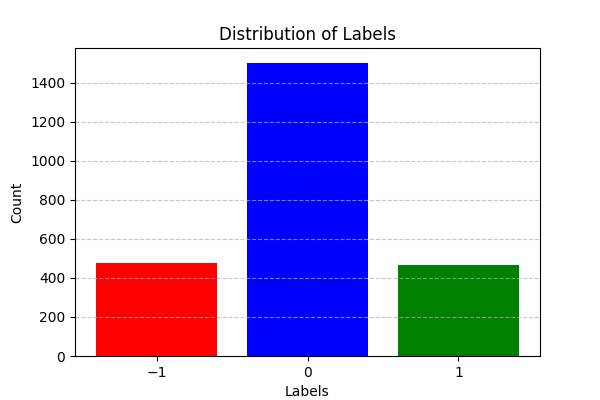
\includegraphics[width=0.8\textwidth]{Figure_1.png}
    \caption{Distribution of labels.}
    \label{fig:sample}
\end{figure}
\noindent
This visualization showcases the distribution of data points across each ground truth label. It is evident 
that there is a noticeable imbalance between the neutral label and the positive and negative labels. The 
positive and negative labels contain approximately the same number of data points, with 468 and 476, respectively. 
In contrast, the neutral label has a significantly higher count of 1,504 data points. 

\section*{Create Baseline}
As a group, we chose to use randomly assigned labels as our baseline, as this approach yielded better overall results. This outcome is reasonable given the class imbalance in our dataset. Had we opted for the majority-class baseline, which assigns the most frequent label to each data file, all instances would have been labeled as neutral (zero) since it is the dominant class across our dataset. \\ \\
\noindent
To evaluate model performance, we trained a Feedforward Neural Network on both human-annotated data and randomly labeled data. The results demonstrated a significant performance gap. When trained on human-annotated data, the model achieved an accuracy of approximately 0.64. In contrast, training on randomly labeled data resulted in a much lower accuracy score of 0.33.
\FloatBarrier
\begin{figure}[h]
    \centering
    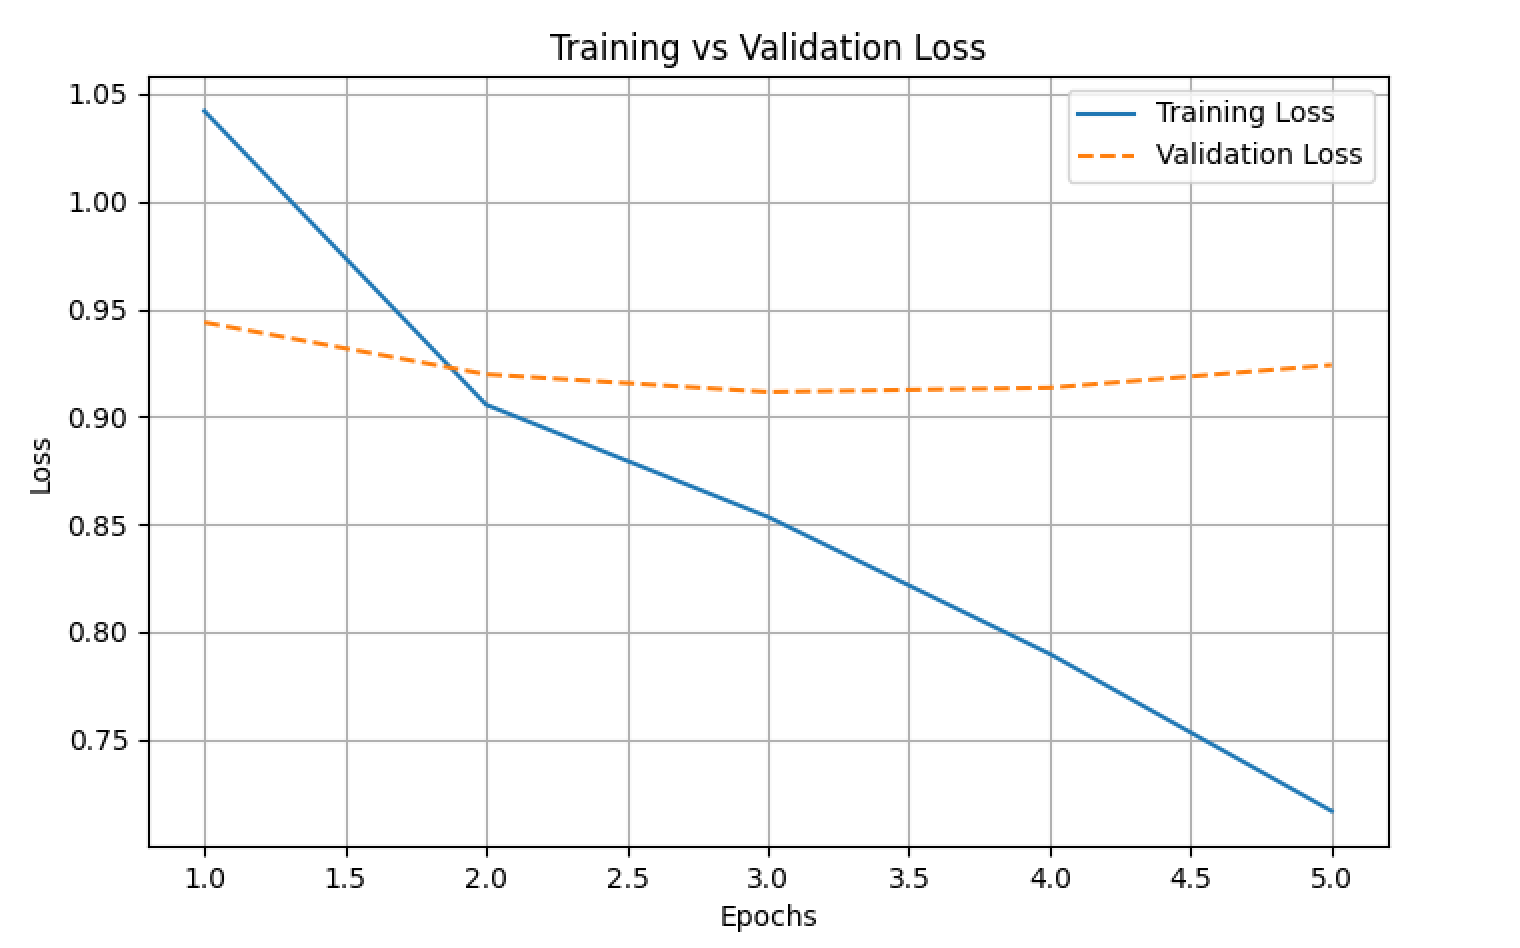
\includegraphics[width=0.8\textwidth]{model.png}
    \caption{Training vs. Validation Loss for the Trained Model.}
    \label{fig:trained_model}
\end{figure}

\begin{figure}[h]
    \centering
    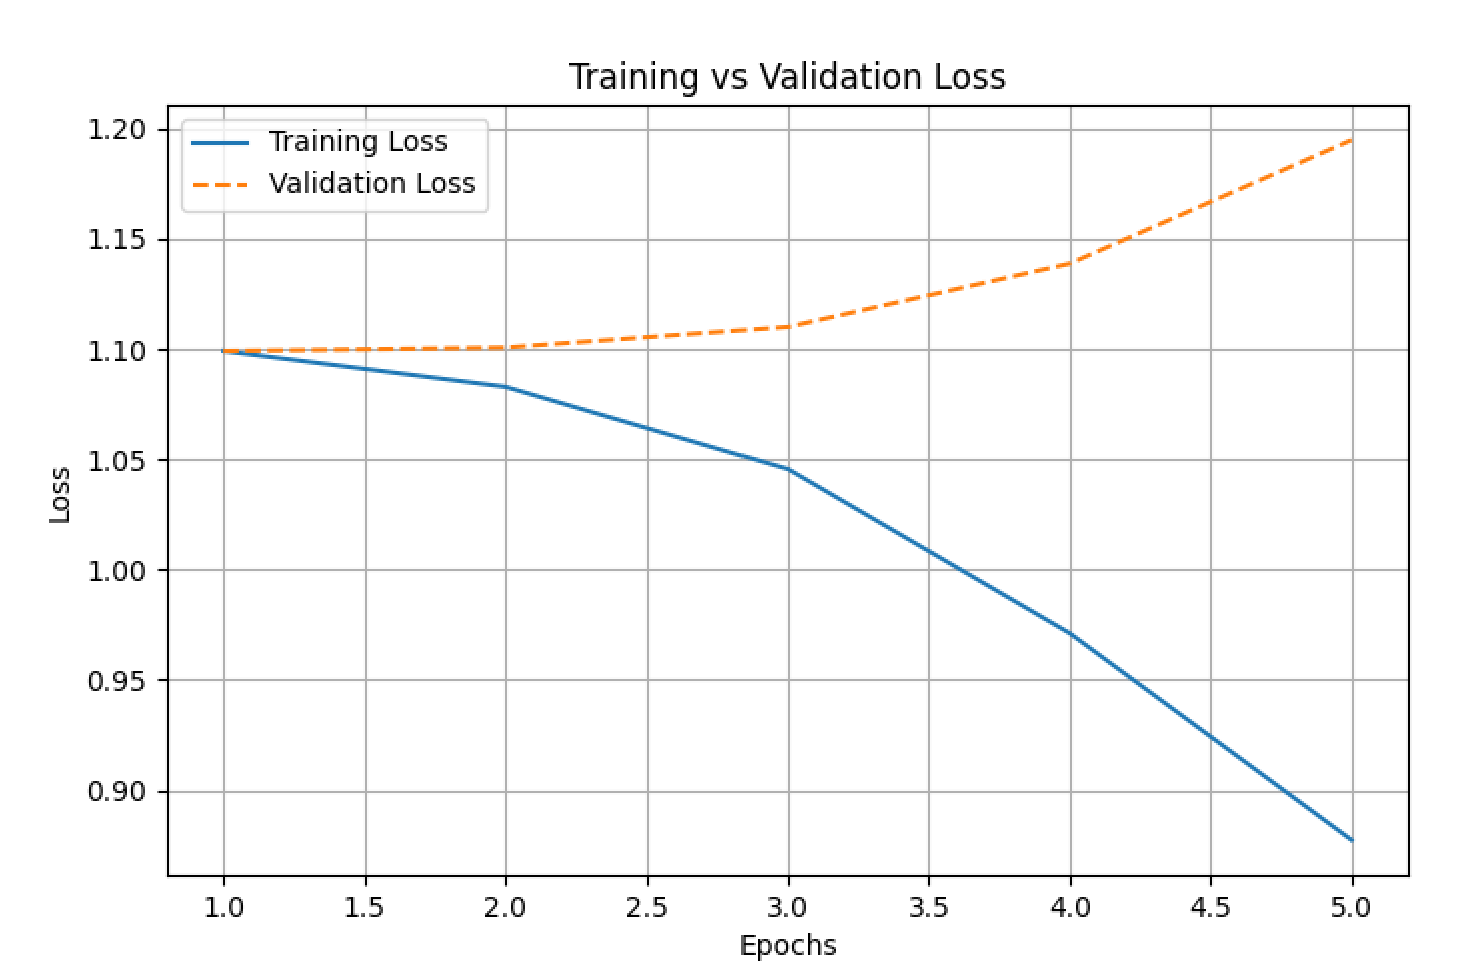
\includegraphics[width=0.8\textwidth]{baseline.png}
    \caption{Training vs. Validation Loss for the Baseline Model.}
    \label{fig:baseline_model}
\end{figure}
\FloatBarrier
\noindent
As observed from the training vs. validation loss graphs, the trained model significantly outperforms the baseline model.

\section*{Conclusion}
 
To further improve the performance of our Feedforward Neural Network in the text classification task, we could explore alternative feature extraction techniques. Currently, we use TF-IDF for feature extraction, but in the future, implementing a word embedding model with mean-pooled embeddings could yield better results. \\ \\
\noindent
Additionally, further tuning of the neural network's hyperparameters—such as the number of hidden dimensions, epochs, and learning rate—could enhance model performance.

\section*{Google Slide Link}

\section*{Codabench Link}
Both of the following Codabench links allow you to run a benchmark using your model's output labels for the test set. \textbf{No actual model is required to run the benchmark; only the label outputs generated by running the model locally are needed.}

\begin{itemize}
    \item \textbf{Benchmark on Human Annotated Data:} \\
    Use this link to run a benchmark on the human-annotated data against your own model outputs for the test set: 
    \url{https://www.codabench.org/competitions/6189/}
    
    \item \textbf{Benchmark on Random Baseline Annotated Data:} \\
    Use this link to run a benchmark on the random baseline annotated data against your own model outputs for the test set: 
    \url{https://www.codabench.org/competitions/6192/}
\end{itemize}
\noindent
If you wish to run the benchmark for either dataset (human annotated or random baseline) using a \texttt{model.py} file, you can use the following link:

\begin{itemize}
    \item \textbf{Benchmark with a \texttt{model.py} file:} \\
    Use this link to run a benchmark with your \texttt{model.py} file for either the human annotated or random baseline dataset: 
    \url{https://www.codabench.org/competitions/6181/?secret_key=2c4738bd-fbc5-4263-8bd6-bd7dd1ad9c1a}
\end{itemize}

\end{document}